\section{Introducción}
\subsection{Estructura de Bandas de Semiconductores}
\begin{frame}[t]
\frametitle{Introducci\'on}
\framesubtitle{}
\vspace{-0.5cm}
\begin{tikzpicture}[remember picture, overlay]
\node<1->[anchor = north west, text width =0.7\textwidth, yshift = -0.75cm](txt) at (current page.north west) {
	\begin{tcolorbox}[enhanced,title =Estructura de Bandas,
	fonttitle=\bfseries,
	left=1mm,
	top=1mm,
	bottom=1mm,
	right=1mm,
	width =\textwidth,
	height=2.5cm,
	boxsep = 0cm,
	coltitle=green!25!black,
	attach boxed title to top center={yshift=-2mm,yshifttext=-1mm},
	boxed title style={colframe=green!75!black,
		colback=yellow!50!green}]
	\begin{itemize}
	\item<1-> Dicta el comportamiento de los electrones dentro de un solido
	\item<2-> En un solido $\approx 10^{23}$ atomos\\$\rightarrow$\text{\color{red}problema complejo de muchos cuerpos}
	\item<3-> Hamiltoniano de un solido
	\end{itemize}
	\end{tcolorbox}	
};

\node<1->[anchor=north east,xshift=-2cm,yshift=-1cm] at (current page.north east){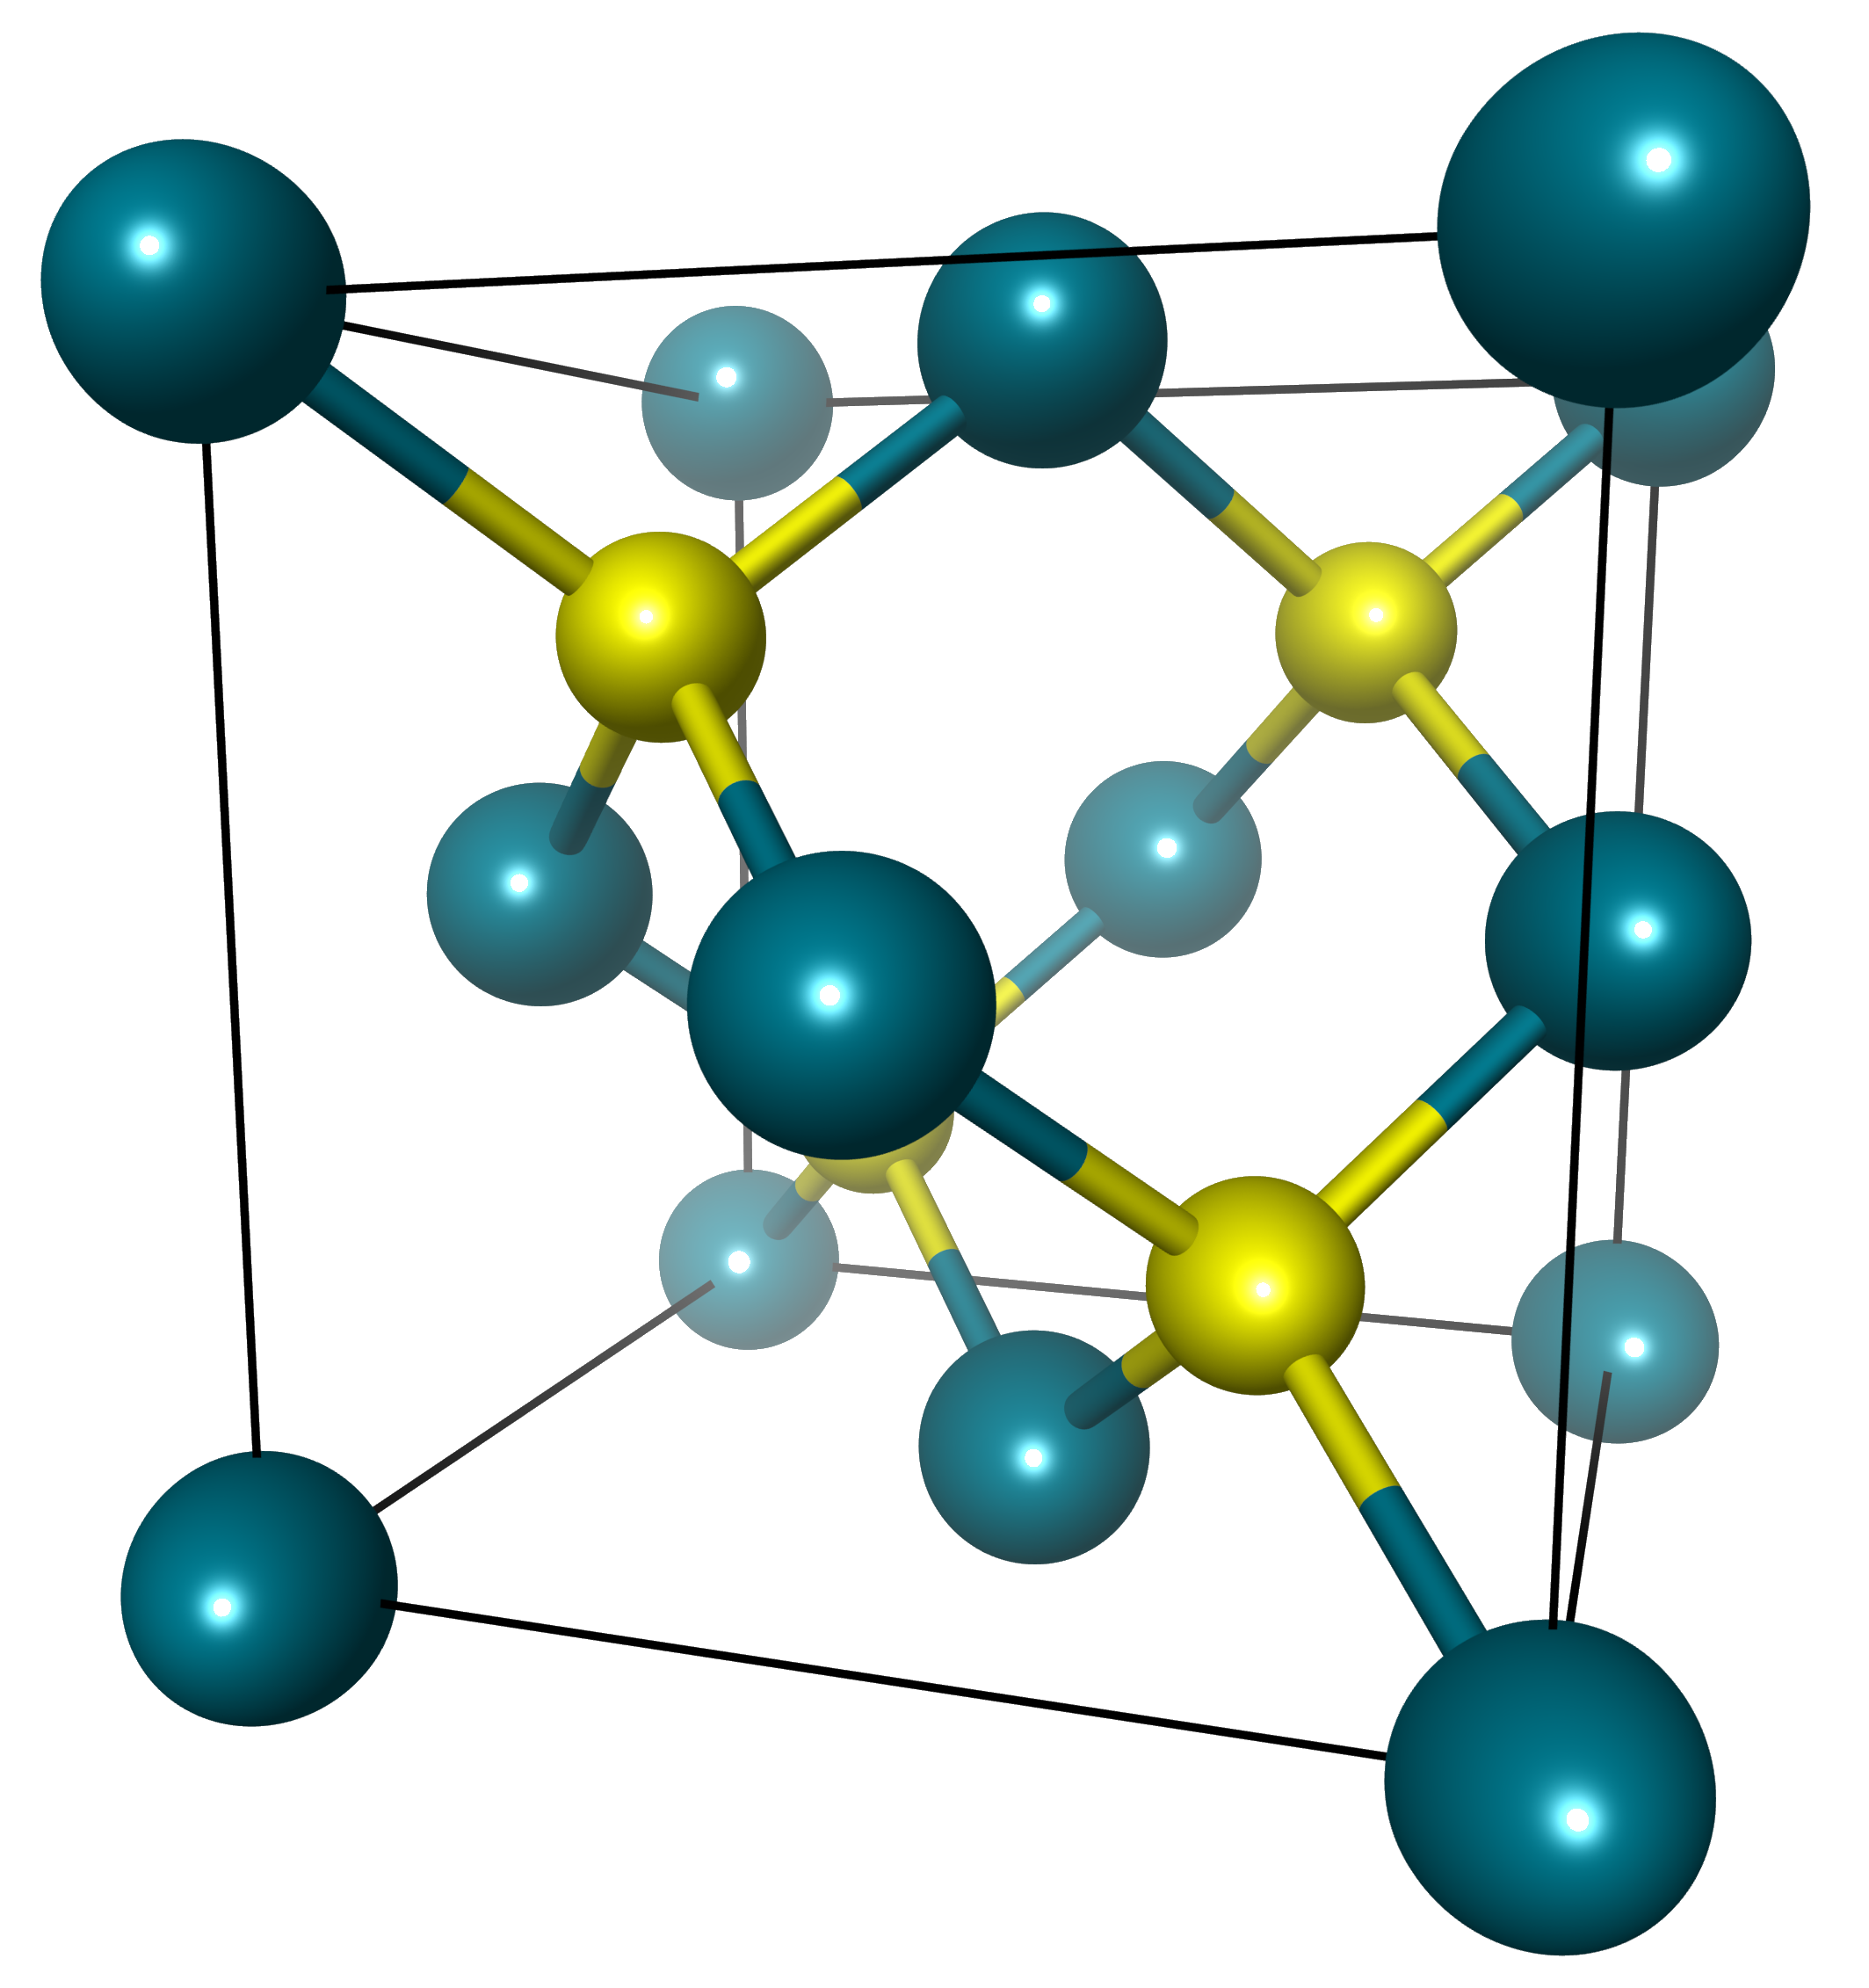
\includegraphics[width=0.35\textwidth]{../../../scripts/structures/GaAs-2}};

\node<3->[anchor=center,text width=\textwidth,font=\sffamily,xshift=-1cm,yshift=-1cm] at (current page.center){
\begin{equation*}
	\begin{split}
	H  =  &\dfrac{1}{2M}\sum\limits_{i=1}^{N_{n}} \bff{P}_{j}^{2} + \dfrac{1}{2m_{0}} \sum\limits_{j=1}^{N_{e}} \bff{p}_{j}^{2} + \dfrac{Z^{2}}{2} \sum\limits_{i,j=1,i\neq j}^{N_{n}} V_{c}\left(\bff{R}_{i}-\bff{R}_{j}\right)-Z\sum\limits_{i=1}^{N_{n}}\sum\limits_{j=1}^{N_{e}}V_{c}\left(\bff{r}_{j}-\bff{R}_{i}\right) \\
	& + \dfrac{1}{2} \sum\limits_{i,j=1,i\neq j}^{N_{e}} V_{c} \left(\bff{r}_{i}-\bff{r}_{j}\right)
	\end{split}
\end{equation*}
};

\end{tikzpicture}
\end{frame}


